\documentclass[russian,utf8,nocolumnxxxi,nocolumnxxxii]{eskdtext}
\usepackage[T1,T2A]{fontenc}
\usepackage[utf8]{inputenc}
\usepackage{amssymb,amsmath}
\usepackage{float}
\usepackage{tikz}
\usepackage{rotating}
\usepackage{graphicx}
\graphicspath{{pictures/}}
\DeclareGraphicsExtensions{.pdf,.png,.jpg}
\usepackage{pgfplots}
\usepackage{lipsum}
\usepackage{nccmath}
\usepackage{siunitx}
\usepackage[european,cuteinductors,smartlabels]{circuitikz}
\usepackage[backend=biber]{biblatex}

\begin{document}

{\bfСодержание}\\
1. Цель и тема курсовой работы\\
2. Задание на курсовую работу\\
3. Введение\\
4. Исследование функции\\
5. Исследование кубического сплайна\\
6. Задача оптимального распределения неоднородных ресурсов\\
7. Список литературы\\
\newpage

 {\large\bf 1. Цель и тема курсовой работы}

{\bfЦель курсовой работы:} уметь применять персональный компьютер и математические пакеты прикладных программ в инженерной деятельности.\\
{\bfТема курсовой работы:} решение математических задач с использованием математического пакета SciLab и системы компьютерной алгебры Reduce.\\

\newpage
{\large\bf2. Задания на курсовую работу}\\
1. Даны функции $f(x)=\sqrt{3}sin(x)+cos(x),g(x)=cos(2x+\frac{\pi}{3})-1$\\
а)Решить уравнение f(x)=g(x).\\
б)Исследовать функцию h(x)=f(x)-g(x) на промежутке $[0;\frac{5\pi}{6}]$\\
2. Найти коэффициенты кубического сплайна, интерполирующего данные, представленные в векторах:\\
$V_{x}=[0,0.5,1,4,2.25,3.5]$\\
$V_{y}=[4,3.7,4.575,4.333,4.167]$\\
Построить на графике функции f(x),полученную после нахождения коэффициентов кубического сплайна. \\
Представить графическое изображение результатов интерполяции исходных данных различными методами с использованием встроенных функций {\bf splin(x,y,“natural”), splin(x,y,“clamped”), splin(x,y,“not\_a\_knot”), splin(x,y, “fast”), splin(x,y,“monotone”), interp(xx,x,y,d)}.\\
3. Решить задачу оптимального распределения неоднородных ресурсов.
Для изготовления {\bf n} видов изделий {\bfИ$_1$}, {\bfИ$_2$} ,... , {\bfИ$_n$} необхо¬димы ресурсы m видов: трудовые, материальные, финансовые и др. Известно тре¬буемое количество отдельного i-гo ресурса для изготовления каждого j-го изделия. Назовем эту величину нормой расхода {\bf C$_i_j$}. Пусть определено количество каждого вида ресурса, которым предприятие располагает в данный момент, - {\bf a$_i$}. Известна прибыль {\bfП$_j$}, получаемая предприятием от изготовления каждого j-го изделия. Требуется определить, какие изделия и в каком количестве должны производиться предприятием, чтобы прибыль была максимальной. 

\begin{figure}[H]
\begin{center}
\begin{minipage}[h]{0.75\linewidth}
\center{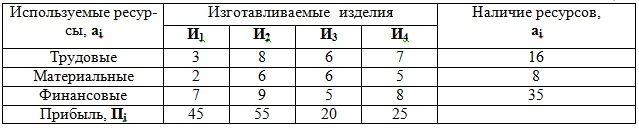
\includegraphics[width=1.\linewidth]{table.jpg}}}  \\
\end{minipage}
\end{center}
\end{figure}


\newpage

{\bf3. Введение}

Профессиональная деятельность инженеров и ученых тесно связана с рассчетами, включающими в себя широкий спектр алгоритмов из различных разделов математики. Ввиду непрагматичности и затратности по времени и ресурсам самостоятельного создания алгоритмов на различных языках программирования, для рассчетов используются специализированные на этом математические пакеты и системы компьютерной алгебры, среди них: MatLab, MathCad, SciLab, SMath, Reduce и другие. Подобный подход позволяет работать с математическими алгоритмами в подготовленной среде с удобным интерфейсом без необходимости на затрату времени на создание кода с нуля. 

\newpage
{\bf4. Исследование функции}\\
1. Даны функции $f(x)=\sqrt{3}sin(x)+cos(x),g(x)=cos(2x+\frac{\pi}{3})-1$\\
а)Решить уравнение f(x)=g(x).\\
б)Исследовать функцию h(x)=f(x)-g(x) на промежутке $[0;\frac{5\pi}{6}]$\\
{\bfРешение уравнения.}\\
Задача а) эквивалентна следующей - требуется найти корни уравнения:\\
$h(x)=\sqrt{3}sin(x)+cos(x)-cos(2x+\frac{\pi}{3})-1$\\
Использование математических пакетов позволяет решать нелинейные уравнения двумя как численно, так и аналитически. Стандартный функционал SciLab позволяет нам получить численное решение, но к сожалению, не способен решить уравнение аналитически напрямую, поэтому для получения второго варианта решения нам придется воспользоваться системой компьютерной алгебры - Reduce.\\
{\bfЧисленное решение с применением SciLab.}\\
При отыскании решения воспользуемся стандартной функцией SciLab - fsolve.\\
Функция h(x), будучи линейной комбинацией периодических функций, обладает периодом равным наименьшему общему кратному периоду этих функций -- $2\pi$. Следовательно, для нахождения периодического решения нелинейного уравнения достаточно будет отыскать корни на отрезке $[0; 2\pi]$. \\
Решение функции fsolve основано на методе касательных и требует заданного интервала или начальной точки для поиска корней уравнения. Для нахождения начальных точек воспользуемся командой plot и построим график функции h(x) на данном отрезке:\\
function y=h(x)\\
y=sqrt(3)*sin(x)+cos(x)-cos(2*x+\%pi/3)+1\\
endfunction\\
plot(0:0.01:2*\%pi,h)\\
График функции отображен на Рис.1.
\newpage

\begin{figure}[H]
\begin{center}
\begin{minipage}[h]{0.65\linewidth}
\center{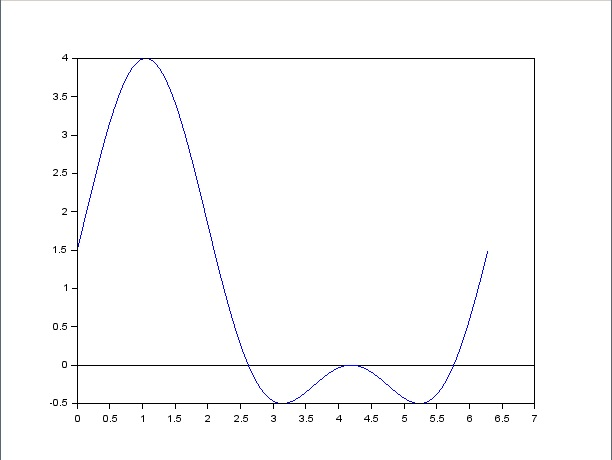
\includegraphics[width=1\linewidth]{scilab_1st.jpg}}}  \\
\frametitle{ Рис 1. График функции h(x)}
\end{minipage}
\end{center}
\end{figure}

Отталкиваясь от от вида графика можно сделать предположение о наличии трех, либо четырех корней, при условии что график дважды пересекает ноль в промежутке x=[4.1;4.3].\\
Воспользуемся функцией fsolve для нахождения точек на графике:\\
$[x,v] = fsolve(x0,f)$, где:\\
x0 – вектор начальных значений для итеративного алгоритма отыскания нулей\\
f – функция, для которой осуществляется поиск нулей\\
x – вектор нулей функции, полученных при работе алгоритма из точек x0\\
v – вектор значений функции в точках x\\
Для проверки предположения о двойном пересечении графиком нуля в промежутке x=[4.1;4.3], укажем две начальных точки поиска с разных сторон от локального максимума, находящегося около x=4.2\\
Строки кода:\\
x0 = [3,3.9,4.5,5.5];\\
$[x,v] = fsolve(x0,h)$\\
v =\\
-2.220D-16 0. 0. 7.772D-16\\
x =\\
2.6179939 {\bf4.1887902} {\bf4.1887902} 5.759865

Полученные точки изображены на Рис.2.
\begin{figure}[H]
\begin{center}
\begin{minipage}[h]{0.65\linewidth}
\center{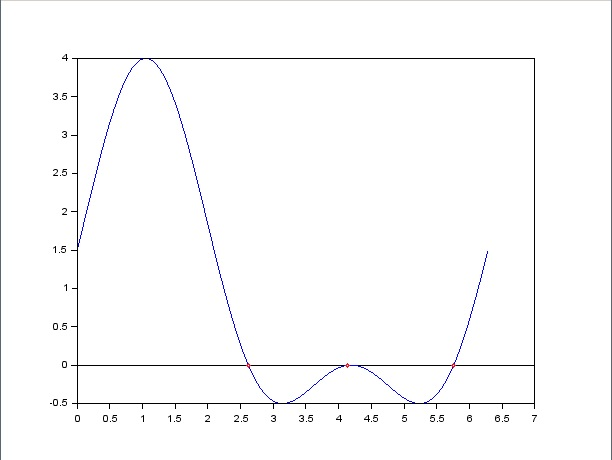
\includegraphics[width=1\linewidth]{scilab_2st.jpg}}}  \\
\frametitle{Рис 2. График функции h(x) с корнями}
\end{minipage}
\end{center}
\end{figure}
\\
Согласно полученным значениям v, два решения не являются нулевыми, ввиду наличия определенной погрешности при решении с применением  fsolve. Также мы убедились, что функция не имеет четвертого корня на заданном отрезке.\\

Корни уравнения имеют следующий вид:\\
$$x_1=2.6179939+2n\pi,n\inZ$$
$$x_2=4.1887902+2n\pi,n\inZ$$
$$x_3=5.759865+2n\pi,n\inZ$$

Принимая во внимание тот факт, что корни линейной комбинации функций sin и cos могут быть кратны $\pi$, разделим полученные корни на данное значение:

x/\%pi =
0.8333333 1.3333333 1.3333333 1.8333333
Полученные десятичные дроби, как видно, кратны 1/3:
3*x/\%pi =
\\2.5 4. 4. 5.5
\newpage
В таком случае, корни приводятся к следующему виду:
$$x_1=\frac{5}{6}*\pi+2n\pi,n\in Z$$
$$x_2=\frac{8}{6}*\pi+2n\pi,n\in Z$$
$$x_3=\frac{11}{6}*\pi+2n\pi,n\in Z$$
Таким образом, используя несложные манипуляции мы перешли от численного решения к аналитическому.\\
\\
{\bfАналитическое решение с применением Reduce.}\\

Для нахождения аналитического решения уравнения воспользуемся функцией solve из системы компьютерной алгебры Reduce:\\
solve(expr,var); где\\
expr – система уравнений\\
var – список из переменных, относительно которых решаются уравнения expr\\

При попытке решить уравнение h(x)= 0 относительно x:\\
solve(sqrt(3)sin(x)+cos(x)-cos(2x+pi/3)-1,x);\\
Решение получено не было.\\
Упростим данное уравнение, воспользовавшись двумя тригонометрическими тождествами: $$sin(x+y)=sin(x)cos(y)+cos(x)sin(y)$$
$$cos(2x)=1-2sin^2(x)$$
$$\sqrt{3}sin(x)+cos(x),g(x)-cos(2x+\frac{\pi}{3})+1$$ $$=2(sin(x)cos(\frac{\pi}{6})+cos(x)sin(\frac{\pi}{6}))+2sin^2(x+\frac{\pi}{6})$$ $$=2(sin(x+\frac{\pi}{6})+sin^2(x+\frac{\pi}{6})$$\\
и получим упрощенное уравнение, эквивалентное исходному
$$2(sin(x+\frac{\pi}{6})+sin^2(x+\frac{\pi}{6})=0$$
Применим к нему функцию solve:\\
solve(2sin(x+pi/6)*(1+sin(x+pi/6)));
и получим решение:
\newpage

\begin{figure}[H]
\begin{center}
\begin{minipage}[h]{0.65\linewidth}
\center{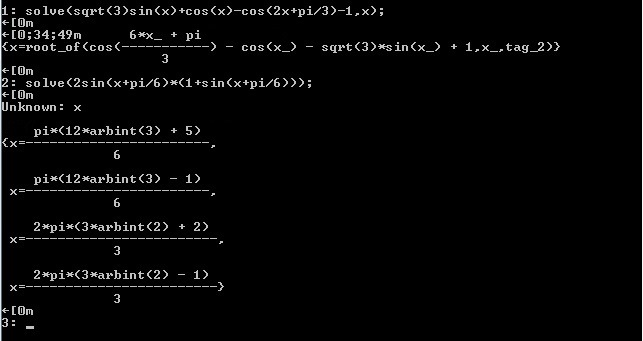
\includegraphics[width=1\linewidth]{reduce.jpg}  \\
\frametitle{Ход решения уравнения с помощью Reduce}
\end{minipage}
\end{center}
\end{figure}


Где arbint является произвольным целым числом. Так как Reduce имеет своеобразный интерфейс, перепишем решение в привычную для нас форму:

$$x_1=\frac{5}{6}*\pi+2n\pi,n\in Z$$
$$x_2=-\frac{1}{6}*\pi+2n\pi,n\in Z$$
$$x_3=\frac{8}{6}*\pi+2n\pi,n\in Z$$
$$x_4=-\frac{4}{6}*\pi+2n\pi,n\in Z$$\\
Периодические решения для $x_3$ и $x_4$совпадают, а периодическое решение для $x_2$ можно записать в виде:
$$x_2=\frac{11}{6}*\pi+2n\pi,n\in Z$$\\
Таким образом, с приненением двух различных математических пакетов и различных подходов были найдены корни нелинейной функции.

\end {document}
